\documentclass[lang=cn,10pt,green]{elegantbook}
\usepackage{float}
\usepackage{subfigure}
\usepackage[normalem]{ulem} % \sout{想加删除线的中文}
\usepackage{wrapfig}
\usepackage{extarrows}
\newcommand{\incfig}[1]{%
\def\svgwidth{\columnwidth}
\import{./figures/}{#1.pdf_tex}
}



\renewcommand{\proofname}{\indent Pr}

\newcommand{\argmin}[1]{\underset{#1}{\arg \min}\ }
\newcommand{\ceil}[1]{\left\lceil #1 \right \rceil }
\newcommand{\norm}[1]{\left \Vert #1 \right \Vert}
\newcommand{\tform}[1]{\left \Vert #1 \right \Vert_2}
\newcommand{\tnorm}[1]{\left \Vert #1 \right \Vert_2}
\newcommand{\onorm}[1]{\left \Vert #1 \right \Vert_1}
\newcommand{\abs}[1]{\left|#1 \right|}
\newcommand{\var}[1]{\text{Var}\left[ #1\right]}
\newcommand{\xk}[1]{\left( #1\right)} 
\newcommand{\zk}[1]{\left[ #1\right]} 
\newcommand{\dk}[1]{\left\{ #1\right\}} 
\newcommand{\bd}[1]{\bold{#1}}

%量子力学符号------
\newcommand{\xde}{\text{Schrödinger}}
\newcommand{\avg}[1]{\left \langle #1 \right \rangle}
\newcommand{\lvec}[1]{\left \langle #1 \right |}
\newcommand{\rvec}[1]{\left | #1 \right \rangle}


\newtheorem{lproof}{证明}[section]
\newtheorem{tuilun}{推论}
\newtheorem{eg}{例}[section]
\newtheorem{solve}{解}[section]
\newcommand\ii{\textup{i}}
\newcommand\dd{\mathrm{d}}


%自定义数学符号
\newcommand{\diag}{\textup{diag}}
\newcommand{\Frobenius}[1]{\left\Vert #1 \right\Vert}
\newcommand{\fform}[1]{\left\Vert #1 \right\Vert_F}
\newcommand{\parr}[2]{\frac{\partial #1}{\partial #2}}%一阶偏微分
\newcommand{\parrr}[2]{\frac{\partial^2 #1}{\partial #2^2}}%二阶偏微分
\newcommand{\lap}[1]{\parrr{#1}{x} + \parrr{#1}{y} = 0}%二元拉普拉斯方程
\newcommand{\ddd}[2]{\frac{\textup{d} #1}{\textup{d} #2}}%微商
\newcommand{\dddd}[2]{\frac{\textup{d}^2 #1}{\textup{d} #2^2}}%微商

%二重以上环路积分,强迫症了属于是
\def\ooint{{\bigcirc}\kern-11.5pt{\int}\kern-6.5pt{\int}}
\def\oooint{{\bigcirc}\kern-12.3pt{\int}\kern-7pt{\int}\kern-7pt{\int}}


\newcommand{\tu}{\textup}
\newcommand{\ol}[1]{$\overline{#1}$}
\newcommand{\re}[1]{\textup{Re}(#1)}
\newcommand{\im}[1]{\textup{Im}(#1)}
\newcommand{\fa}{\forall}
\newcommand{\ex}{\exists}
\newcommand{\st}{\textup{  s.t. }}
\newcommand{\ve}{\varepsilon}
\newcommand{\disp}{\displaystyle}
\newcommand{\chj}{\textup{Cauchy}积分公式}
\newcommand{\res}[1]{\textup{Res}\left(#1\right)}
\newcommand{\mysum}[1][n]{\sum_{i = 1}^{#1}}%求和
\newcommand{\series}[1]{\sum_{n = 0}^{\infty} #1_{n}}%级数
\newcommand{\seriesa}[1]{\sum_{n = 0}^{\infty} \left| #1_{n}\right|}%绝对级数
\newcommand{\fseries}[1]{\sum_{k = 1}^{\infty} #1_k (z)}

\newcommand*{\num}{pi}

%书写横线
\newcommand{\horrule}[1]{\rule[0.5ex]{\linewidth}{#1}} 	% Horizontal rule

\title{Introduction to Computer Vision Notes}
\subtitle{授课教师:\href{https://hughw19.github.io}{王鹤}}
\author{林晓疏, \href{https://lyt0112.com/}{梁宇桐}, \href{https://iculizhi.github.io/}{徐靖},\href{https://arthals.ink/}{卓致用}}
\institute{PKU EECS}
\version{2025 Spring}
\bioinfo{声明}{\textcolor{red}{请勿用于个人学习外其他用途!}}
\extrainfo{个人笔记,如有谬误,欢迎指正!\\ 联系方式:2200012917@stu.pku.edu.cn}

\setcounter{tocdepth}{3}

% 自定义封面元素
\cover{cover.jpg}
\logo{logo-blue.png}

% 本文档命令
\usepackage{array}
\newcommand{\ccr}[1]{\makecell{{\color{#1}\rule{1cm}{1cm}}}}

% 修改标题页的橙色带
\definecolor{customcolor}{RGB}{214, 136, 0}
\colorlet{coverlinecolor}{customcolor}
\setcounter{tocdepth}{3} % 设置目录深度
\begin{document}

\maketitle
\frontmatter

\tableofcontents

\mainmatter

\chapter{Deep learning 1}
\begin{introduction}[keywords]
    \item Feature extraction : 特征提取
    \item Logistic Regression : 逻辑回归
    \item Heuristic model : 启发式模型
    \item Maximum Likelihood Estimation : 最大似然估计
    \item Stochastic Gradient Descent : 随机梯度下降
    \item Multilayer Perceptron : 多层感知机
    \item Dense layer : 全连接层
\end{introduction}
\section{Feature Description}

\begin{problem}
    我们已经知道了如何去 detect 一些点, 下一步如何通过描述他们进行匹配呢?
\end{problem}

    将图像内容转换为不受平移、旋转、缩放和其他成像参数影响的局部特征坐标. 例如, 房子的地点, 大小, 风格, 建造时间, 当前状况等. 基于这些 features, 我们有:
    \begin{itemize}
        \item Heuristic model (启发式模型): $y = (10-\text{location})\times \text{area}$
        \item Parametric model (参数模型): $y = \phi_\theta(F)$
    \end{itemize}
\begin{note}
拥有一些 observations 后, 我们就可以 fit $\theta$.
\end{note}

\section{Machine learning}

当我们有了一组 observations $\{(x_i, y_i)\}_{i=1}^N$, 我们希望找到 $y$ 和 $x$ 的关系.
\begin{itemize}
    \item Line fitting: 我们知道这个关系近似为线性关系, 所以用 $y = mx + b$ 来拟合.
    \item Training neural network: 我们用参数模型来拟合, 但是我们对其所知甚少.
\end{itemize}
\begin{definition}[Outline]
    \begin{itemize}
        \item Set up the task
        \item Perpare the data $\to$ Need a labeled dataset
        \item Build a model $\to$ Construct your neural network
        \item Decide the fitting/training objective $\to$ Loss function
        \item Perform fitting $\to$ Training by running optimization
        \item Testing $\to$ Evaluating on test data
    \end{itemize}
\end{definition}

\subsection{Task}
\begin{figure}[htbp]
    \centering
    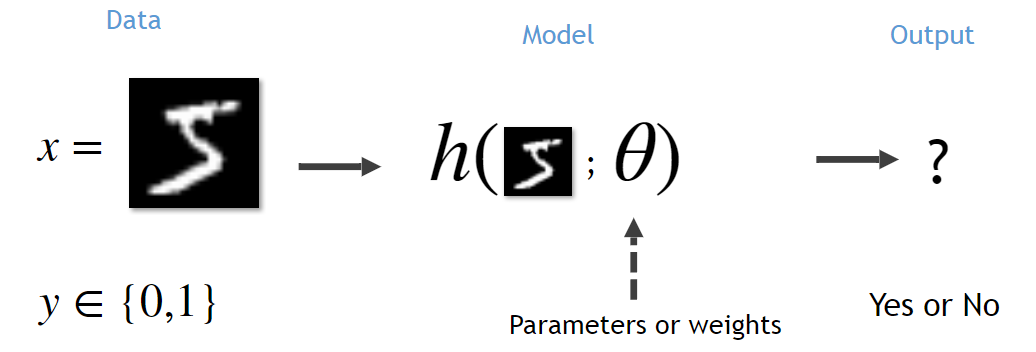
\includegraphics[width=0.8\textwidth]{figures/ministdataset.png}
    \caption{pipeline}
    \label{fig:ml-pipeline}
\end{figure}

\clearpage

\subsection{Data}

\begin{figure}[htbp]
    \centering
    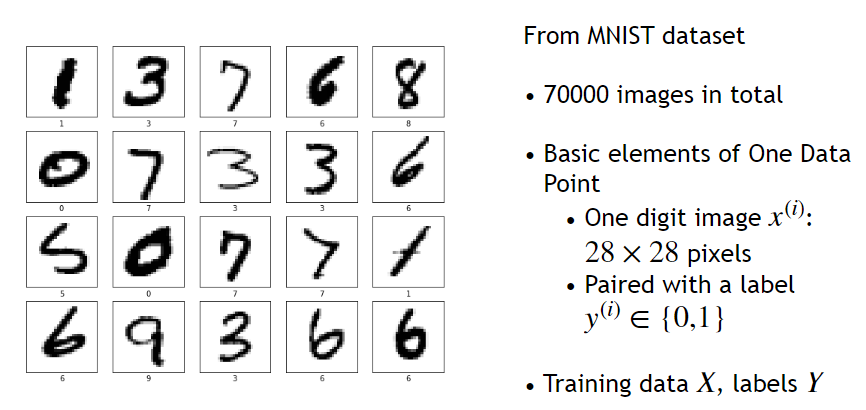
\includegraphics[width=0.8\textwidth]{figures/Mnistdataset.png}
    \caption{MINIST Dataset}
    \label{fig:ml-dataset}
\end{figure}

\subsection{Model}
我们使用所谓逻辑回归 (Logistic Regression) 来进行分类, 其模型为:
$$h(x) = g(\theta^T x) = \frac{1}{1 + e^{-\theta^T x}}$$
\begin{note}
    这里的 $g$ 是 sigmoid 函数 $g(z) = \frac{1}{1 + e^{-z}}$, 将 $z\in \mathbb{R}$ 映射到 $[0, 1]$, 提供非线性性.
\end{note}
\subsection{Loss function}
\begin{definition}[最大似然估计]
    \begin{itemize}
        \item 即最大化似然函数, 使得在假定的统计模型下, 观察到的数据是最有可能的.
        \item 参数空间中最大化似然函数的点 (实际上是网络权重) 称为最大似然估计.
    \end{itemize}
\end{definition}
回到原任务, 我们有:
$$ p(y|x, \theta) = h_{\theta}(x)^y (1 - h_{\theta}(x))^{1-y} $$
\begin{note}
    这里 y 取值为 0 或 1, x 是 28x28 的图像, $\theta$ 是我们要学习的参数
\end{note}
自然地假设所有数据点独立同分布, 因此我们有:
$$ p(Y|X, \theta) = \prod_{i=1}^N p(y_i|x_i, \theta) = \prod_{i=1}^N h_{\theta}(x_i)^{y_i} (1 - h_{\theta}(x_i))^{1-y_i} $$

Loss 就是我们想去最小化的东西, 这里可以有所谓 Negative Log Likelihood (NLL) loss :
$$ \mathcal{L}({\theta}) = -\log p(Y|X, \theta) = -\sum_{i=1}^N \left( y_i \log h_{\theta}(x_i) + (1 - y_i) \log (1 - h_{\theta}(x_i)) \right) $$
\clearpage
\subsection{Training : Gradient Descent}
此时我们可以去定义一个优化问题, 但通用的优化问题是困难的, 有一些问题类型可以被有效地解决, 例如:
\begin{itemize}
    \item Convex optimization: 目标函数是一个凸函数, 约束条件是一个凸集.
    \item Linear programming: 目标函数是线性的, 约束条件是线性的.
    \item Least squares: 目标函数是二次函数, 约束条件是线性的.
\end{itemize}
如果我们将参数空间放到横轴, Loss 放到纵轴, 我们可以自然地得到一个曲面 (这是Loss具备的数学性质), 对于曲面自然存在凸性的局部或者整体:

% 将loss1.png和loss2.png左右排布放在一起, 高度对齐

\begin{figure}[htbp] 
        \centering
        \begin{minipage}[b]{0.45\linewidth}
            \centering
            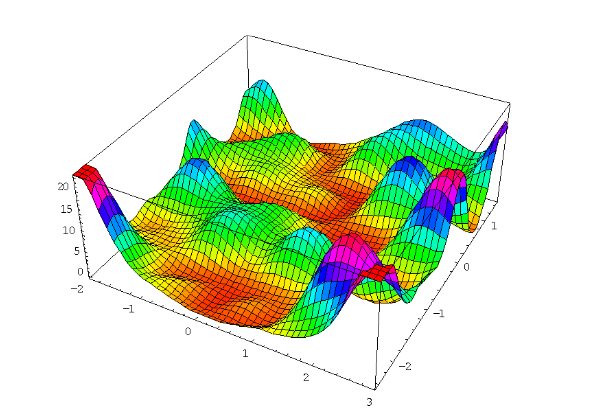
\includegraphics[width=\textwidth]{figures/loss1.png}
            \caption{Non-convex energy landscape}
            \label{fig:loss1}
        \end{minipage}
        \hfill
        \begin{minipage}[b]{0.3\linewidth}
            \centering
            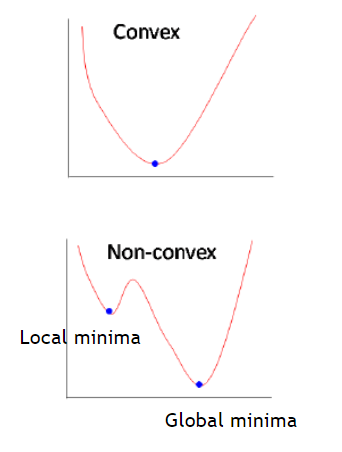
\includegraphics[width=\textwidth]{figures/loss2.png}
            \caption{minima}
            \label{fig:loss2}
        \end{minipage}
\end{figure}

\begin{definition}[Gradient Descent]
    \begin{itemize}
        \item 每次迭代的公式 :
        $$\theta_{t+1} = \theta_t - \alpha \nabla_{\theta} \mathcal{L}(\theta_t)$$
        \item 其中 $\alpha$ 是学习率, $\nabla_{\theta} \mathcal{L}(\theta_t)$ 是 Loss 的梯度.
    \end{itemize}
\end{definition}

\begin{note}
而对于我们的 NLL loss, 注意到 sigmoid 函数有 $g'(z) = g(z)(1-g(z))$, 我们可以得到 :
$$\begin{aligned}\frac{\partial\mathcal{L}}{\partial\theta_{j}}&=-\sum\left(y\frac1{g(\theta^Tx)}-(1-y)\frac1{1-g(\theta^Tx)}\right)\frac\partial{\partial\theta_j}g(\theta^Tx)\\&=-\sum\left(y\frac1{g(\theta^Tx)}-(1-y)\frac1{1-g(\theta^Tx)}\right)g(\theta^Tx)(1-g(\theta^Tx))\frac\partial{\partial\theta_j}\theta^Tx\\&=-\sum\left(y(1-g(\theta^Tx))-(1-y)g(\theta^Tx)\right)x_j\\&=-\sum\left(y-h_\theta(x)\right)x_j\end{aligned}
$$
\end{note}
\begin{theorem}[Stochastic Gradient Descent]
    所谓的 Batch Gradient Descent 是指每次迭代都使用所有的训练数据来计算梯度, 但是这样会非常慢, 因此我们可以使用 Stochastic Gradient Descent (SGD), 每次迭代只使用随机出的 N 对样本. 此时令:
    $$\nabla_{\theta} \mathcal{L}(\theta_t) = \frac{1}{N}\sum_{i=1}^N \nabla_{\theta} \mathcal{L}(\theta_t, x_i, y_i)$$
    此外, SGD 有助于跳出 local minima, 但是会导致 loss 函数震荡.
\end{theorem}

\subsection{Testing}
训练后, 我们需要测试泛化性, 也就是模型在未见过的数据上的表现.

\section{Multilayer Perceptron\footnote{MLP 是非常经典且优美的神经网络, 笔者做生成式模型, 能看到即便在当前很前沿的研究中, 也会用到 MLP, 例如著名的 Nerf 方法}}
\begin{note}
    单层网络解决不了线性不可分的问题, 因此我们需要 MLP. 
\end{note}

\begin{figure}[htbp]
    \centering
    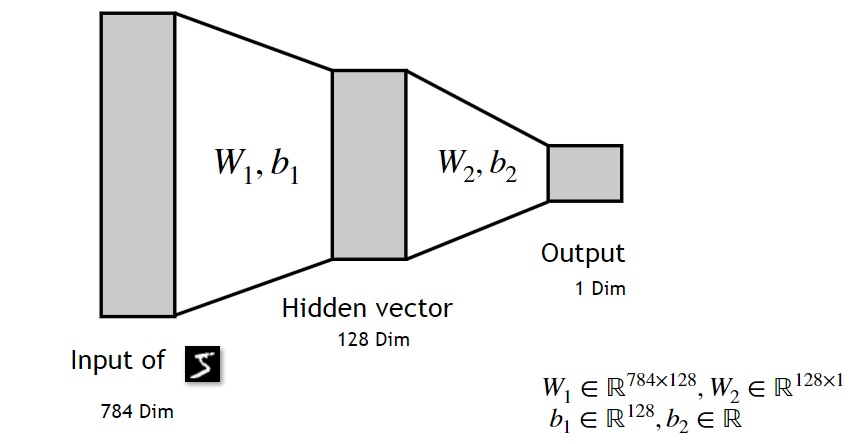
\includegraphics[width=0.8\textwidth]{figures/mlp.png}
    \caption{MLP 前向过程示例}
    \label{fig:mlp}
\end{figure}
$$ f(x; \theta) = g(W_2 g(W_1 x + b_1) + b_2) $$


\subsection{Chain Rule}
\begin{problem}
    如何训练 MLP? 如何获取梯度?
\end{problem}
使用矩阵计算链式法则的结果解决这个问题, 得到每个参数 $W_i, b_i$ 的梯度, 那就可以更新参数了. 我们判断一个网络是否可以更新, 一个直观的标准就是看他的前向过程是否可微可导. 即便实际操作未必参与计算. 
\begin{figure}[htbp]
    \centering
    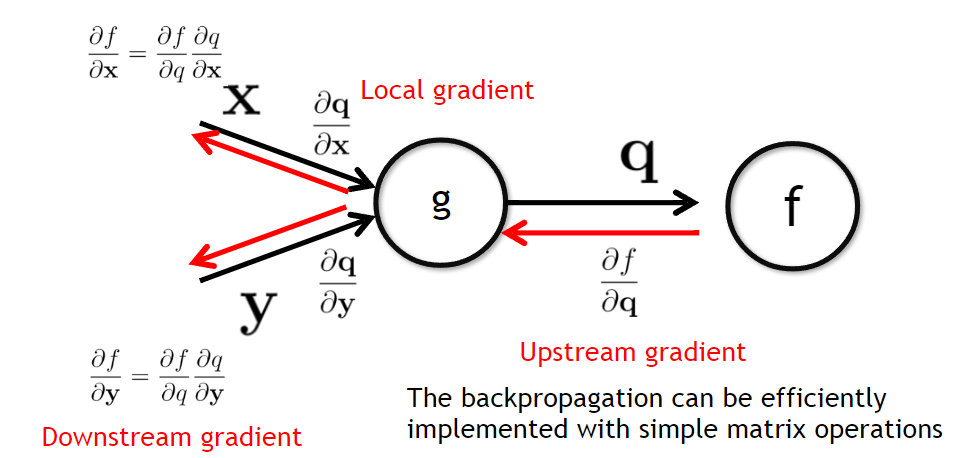
\includegraphics[width=0.8\textwidth]{figures/chainrule.png}
    \caption{链式法则求梯度}
    \label{fig:chainrule}
\end{figure}

\subsection{Activation function}

\begin{figure}[htbp]
    \centering
    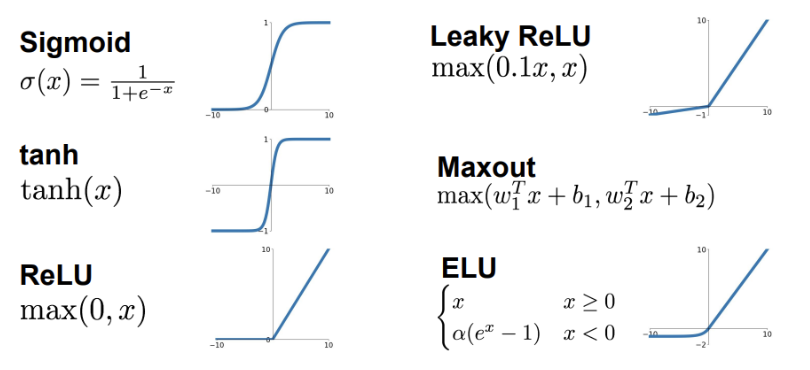
\includegraphics[width=0.8\textwidth]{figures/activationfunc.png}
    \caption{常用激活函数}
    \label{fig:chainrule}
\end{figure}

\begin{note}
激活函数替代我们的 $g$, 其中 ReLU 通常是大部分问题的默认选择
\end{note}

\begin{definition}[Fully connected layer]
    \begin{itemize}
        \item 每个神经元都和前一层的每个神经元相连, 也叫做 Dense layer.
    \end{itemize}
\end{definition}

\subsection{Problems of MLP}
视觉信号过程中, MLP 可能会遇到一些问题:
\begin{itemize}
    \item 计算量大, 将高分辨率图像向量化非常耗时.
    \item 扁平化操作会破坏图像的局部结构.
\end{itemize}

\clearpage
% appendix: appendix-QRDecomposition, condition-number, transformation-in-space

\printbibliography[heading=bibintoc, title=\ebibname]
\end{document}
